\documentclass[11pt,a4paper]{article}
\usepackage[utf8]{inputenc}
\usepackage[T1]{fontenc}
\IfFileExists{spanish.ldf}{\usepackage[spanish]{babel}}{\renewcommand{\figurename}{Figura}\renewcommand{\tablename}{Tabla}\renewcommand{\appendixname}{Apéndice}\renewcommand{\abstractname}{Resumen}}
\usepackage{amsmath,amssymb}
\usepackage{graphicx}
\usepackage{booktabs}
\usepackage{listings}
\usepackage{xcolor}
\usepackage{float}
\usepackage[margin=2.5cm]{geometry}
\newcommand{\cOpsK}{2.93}
\newcommand{\cTK}{9.49}
\newcommand{\cOpsB}{13.35}
\newcommand{\cTB}{6.04}
\newcommand{\errOpsK}{12}
\newcommand{\errTK}{9}
\newcommand{\errOpsB}{9}
\newcommand{\errTB}{29}
\newcommand{\nKruskalMax}{1000000}
\newcommand{\mKruskalMax}{3000000}
\newcommand{\tKruskalMax}{0.65}
\newcommand{\tBrutaDiez}{43.5}
\newcommand{\factorNueveDiez}{28.2}


\lstset{
  language=C++, basicstyle=\ttfamily\footnotesize, numbers=left, numberstyle=\tiny,
  breaklines=true, frame=single, columns=fullflexible, keepspaces=true,
  commentstyle=\color{gray}, keywordstyle=\color{blue},
  literate={á}{{\'a}}1 {é}{{\'e}}1 {í}{{\'i}}1 {ó}{{\'o}}1 {ú}{{\'u}}1 {ñ}{{\~n}}1 {Á}{{\'A}}1 {É}{{\'E}}1 {Í}{{\'I}}1 {Ó}{{\'O}}1 {Ú}{{\'U}}1
}

\title{Árbol de mínima cobertura: Kruskal frente a fuerza bruta\\\large Análisis y Diseño de Algoritmos}
\author{María Paz Puerta Acevedo}
\date{Martes 17 de noviembre de 2026}

\begin{document}
\maketitle

\section{Problema elegido}
Se eligió el problema del \emph{árbol de mínima cobertura} (MST). Dado un grafo no dirigido y conexo $G=(V,E)$ con $n$ nodos, $m$ arcos y un costo $c_e$ para cada arco, se busca un árbol de cobertura $T$ cuya suma de costos sea la menor posible.

\section{Algoritmos implementados}
\subsection{Algoritmo eficiente: Kruskal}
Se implementó el algoritmo de Kruskal visto en clase, con el mismo pseudocódigo de la diapositiva:
\begin{itemize}
  \item Ordenar los $m$ arcos por costo.
  \item $T=\emptyset$ y \texttt{make-set}$(v)$ para cada nodo $v$.
  \item Para cada arco $e_i=(u,v)$ en orden: si \texttt{find-set}$(u)\neq$ \texttt{find-set}$(v)$, agregar $e_i$ a $T$ y hacer \texttt{union}$(u,v)$.
\end{itemize}
Para \texttt{union-find} se usa un arreglo \texttt{padre} con compresión de caminos. El ordenamiento se hace con \texttt{sort} de C++. Como se vio en clase, Kruskal es un caso especial del algoritmo codicioso con las reglas roja y azul, y por eso produce un MST. Al final, si $T$ no tiene $n-1$ arcos, el grafo no es conexo y el programa lo avisa.

\subsection{Fuerza bruta}
Se prueban todos los subconjuntos de $n-1$ arcos entre los $m$ que hay. Para cada subconjunto se revisa si algún arco forma un ciclo (usando también conjuntos disjuntos). Si no hay ciclos, los $n-1$ arcos forman un árbol de cobertura, y se guarda el de menor costo. Si ningún subconjunto sirve, el grafo no es conexo.

\subsection{Entrada y salida}
Los dos programas se ejecutan como \texttt{./programa entrada.txt salida.txt}. La entrada tiene en la primera línea \texttt{n m}, y luego $m$ líneas \texttt{u v costo} con los nodos numerados de $0$ a $n-1$. La salida tiene el costo del árbol, sus arcos, el número de instrucciones contadas (\texttt{instrucciones}) y el tiempo en nanosegundos (\texttt{tiempo\_ns}). Si el grafo no es conexo se escribe \texttt{grafo no conexo} en vez del costo y los arcos. Los programas también avisan si falta un argumento, si el archivo no existe o si el formato está mal.

\section{Instrumentación}
\paragraph{Instrucciones.} Hay una variable global \texttt{instrucciones}. En los dos programas se sigue la misma regla: se suma 1 por cada instrucción simple que se ejecuta (una asignación, una comparación, la condición de un \texttt{if}, una llamada a función). El encabezado de un \texttt{for} cuenta 1 por iteración. En el ordenamiento de Kruskal se cuenta 1 por cada comparación que hace \texttt{sort}. Es un conteo aproximado, pero siempre da el mismo valor para la misma instancia y sirve para ver cómo crece el algoritmo. Como la regla es igual en los dos programas, sus conteos se pueden comparar.

\paragraph{Tiempo.} Se mide con \texttt{std::chrono::steady\_clock} desde el inicio del algoritmo (después de leer el archivo) hasta su final (antes de escribir el resultado). Como una sola medición puede variar, cada instancia se ejecuta varias veces (entre 3 y 15) y se reporta la mediana.

\section{Generador de instancias}
El programa \texttt{generador} recibe $n$, $m$, una semilla y el nombre del archivo. Primero crea un árbol al azar (cada nodo $v$ se une con un nodo anterior elegido al azar), así el grafo siempre es conexo. Después agrega arcos distintos al azar hasta tener $m$. Los costos son enteros al azar entre $1$ y $10^6$. Con la misma semilla se obtiene siempre la misma instancia.

\section{Experimentos}
La fuerza bruta es muy lenta para tamaños grandes, así que se usaron dos tipos de instancias:
\begin{itemize}
  \item Grafos completos con $n=4,\dots,10$ (es decir, $m=n(n-1)/2$), con los dos algoritmos.
  \item Grafos con $m=3n$ y $n$ desde $10^3$ hasta $10^6$, solo con Kruskal.
\end{itemize}
En todas las instancias donde se ejecutaron los dos algoritmos el costo del MST fue el mismo. Además, el script \texttt{verificar.sh} compara los dos algoritmos en 200 instancias pequeñas al azar y no encontró ninguna diferencia.

\begin{table}[H]
\centering
\begin{tabular}{rrrrr}
\toprule
$n$ & $m$ & Instrucciones & Tiempo (ms) & Kruskal (instr.)\\
\midrule
4 & 6 & 1168 & 0.004 & 125\\
5 & 10 & 14764 & 0.014 & 201\\
6 & 15 & 247367 & 0.162 & 311\\
7 & 21 & 5070544 & 3.067 & 440\\
8 & 28 & 123984630 & 67.590 & 609\\
9 & 36 & 3462754535 & 2188.040 & 769\\
10 & 45 & 111339104729 & 40669.557 & 1004\\
\bottomrule
\end{tabular}

\caption{Fuerza bruta en grafos completos. La última columna son las instrucciones de Kruskal en la misma instancia.}
\end{table}

\begin{table}[H]
\centering
\begin{tabular}{rrrr}
\toprule
$n$ & $m$ & Instrucciones & Tiempo (ms)\\
\midrule
1000 & 3000 & 113921 & 0.326\\
2000 & 6000 & 238002 & 0.686\\
5000 & 15000 & 642139 & 1.838\\
10000 & 30000 & 1362709 & 4.223\\
20000 & 60000 & 2830416 & 8.543\\
50000 & 150000 & 7435821 & 22.163\\
100000 & 300000 & 15446257 & 54.886\\
200000 & 600000 & 32248880 & 109.632\\
500000 & 1500000 & 85344527 & 299.573\\
1000000 & 3000000 & 173569172 & 652.603\\
\bottomrule
\end{tabular}

\caption{Kruskal en grafos con $m=3n$.}
\end{table}

\section{Análisis teórico}
\subsection{Kruskal}
\begin{itemize}
  \item Ordenar los $m$ arcos cuesta $O(m\log m)$.
  \item Hacer \texttt{make-set} para los $n$ nodos cuesta $O(n)$.
  \item El ciclo hace $m$ iteraciones, y en cada una hay dos \texttt{find-set} y a lo sumo una \texttt{union}. Con \texttt{union-find} cada operación cuesta $O(\log n)$, y como el grafo es conexo $n-1\le m$, así que esto es $O(\log m)$. El ciclo cuesta entonces $O(m\log m)$.
\end{itemize}
En total Kruskal es $O(m\log m)$, igual que en la diapositiva. Esta es la función de menor crecimiento posible para este algoritmo, porque ordenar por comparaciones ya necesita al menos del orden de $m\log m$ pasos. Entonces
\[
f_K(m)=m\log m .
\]

\subsection{Fuerza bruta}
Se revisan $\binom{m}{n-1}$ subconjuntos, y cada revisión cuesta $O(n)$ (reiniciar los conjuntos y recorrer a lo sumo $n-1$ arcos). Además, las llamadas de la recursión no pasan de $n\binom{m}{n-1}$. Por eso
\[
f_B(n,m)=n\binom{m}{n-1}.
\]
En un grafo completo $m=n(n-1)/2$ y $\binom{m}{n-1}\ge\left(\frac{m}{n-1}\right)^{n-1}=\left(\frac{n}{2}\right)^{n-1}$, por lo que el costo crece más rápido que cualquier función exponencial $c^n$.

\section{Comparación con los datos}
Para cada algoritmo se buscó una constante $C$ tal que la gráfica de $C\,f(n)$ quede lo más cerca posible de los datos. Se calculó el cociente $\text{dato}/f$ para cada tamaño y se tomó la mediana de esos cocientes. Para el tiempo no se usaron las ejecuciones menores a 1\,ms, porque son tan cortas que casi solo miden ruido; aun así aparecen en las gráficas.
\begin{center}
\begin{tabular}{lcc}
\toprule
Algoritmo & $C$ (instrucciones) & $C$ (tiempo, ns)\\
\midrule
Kruskal, $f_K=m\log_2 m$ & \cOpsK & \cTK\\
Fuerza bruta, $f_B=n\binom{m}{n-1}$ & \cOpsB & \cTB\\
\bottomrule
\end{tabular}
\end{center}

\begin{figure}[H]
\centering
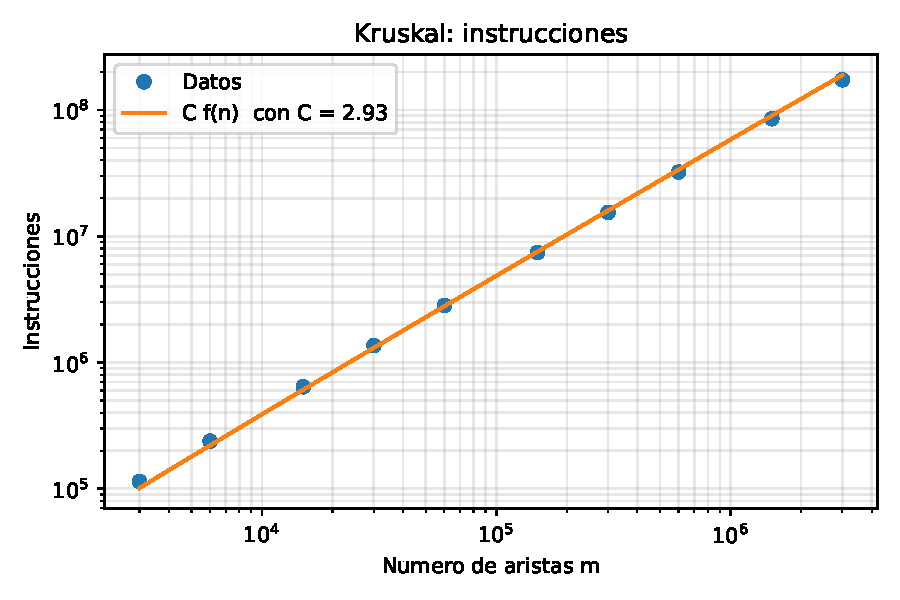
\includegraphics[width=0.48\textwidth]{../graficas/kruskal_ops.pdf}
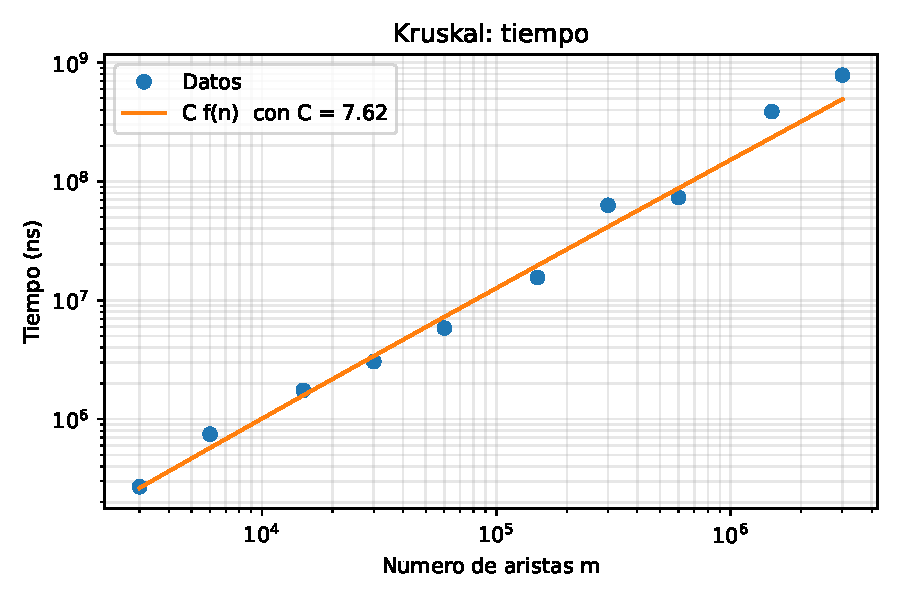
\includegraphics[width=0.48\textwidth]{../graficas/kruskal_tiempo.pdf}
\caption{Kruskal: datos y la curva $C\,m\log_2 m$ (ejes logarítmicos).}
\end{figure}

\begin{figure}[H]
\centering
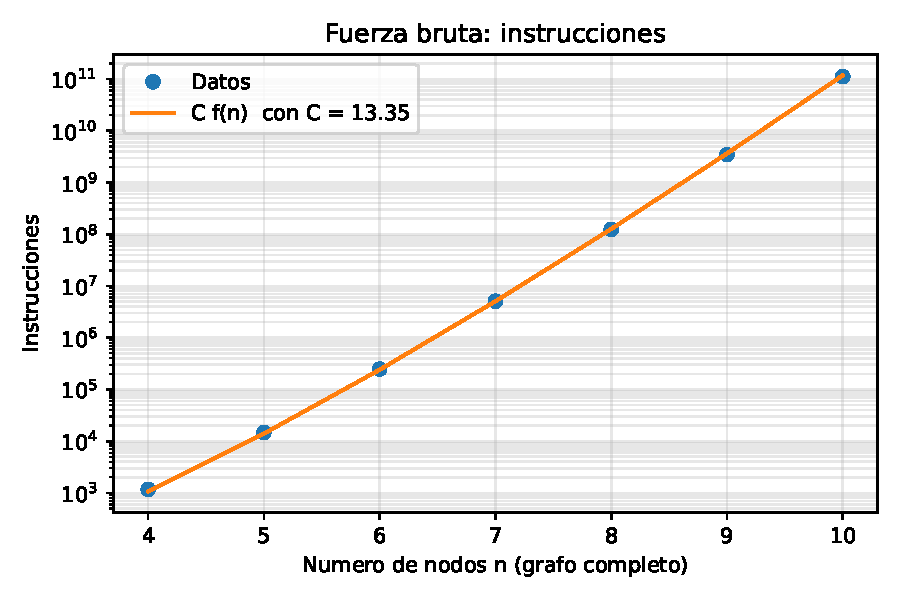
\includegraphics[width=0.48\textwidth]{../graficas/bruta_ops.pdf}
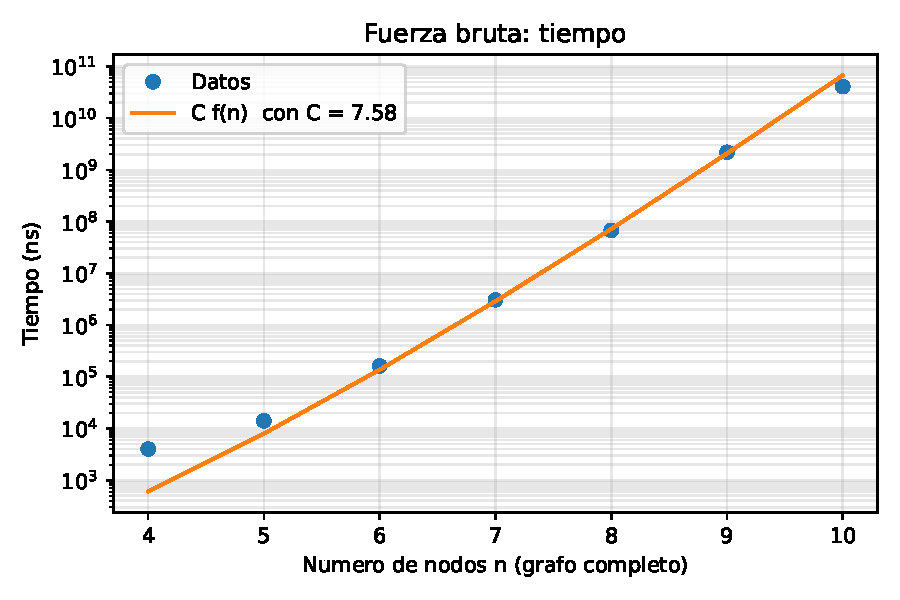
\includegraphics[width=0.48\textwidth]{../graficas/bruta_tiempo.pdf}
\caption{Fuerza bruta: datos y la curva $C\,n\binom{m}{n-1}$ (eje vertical logarítmico).}
\end{figure}

En las gráficas de Kruskal los datos siguen de cerca la curva $C\,m\log_2 m$: la mayor diferencia entre los datos y la curva es de \errOpsK\,\% en instrucciones y de \errTK\,\% en tiempo. Esto confirma que Kruskal se comporta como $m\log m$.

En la fuerza bruta las instrucciones también siguen la curva $C\,n\binom{m}{n-1}$, con una diferencia máxima de \errOpsB\,\%. El tiempo se parece a la curva, pero no tanto: con las ejecuciones de más de 1\,ms ($n\ge 7$) la diferencia máxima es de \errTB\,\%. Para $n$ pequeño las ejecuciones duran microsegundos y el tiempo medido casi no depende del algoritmo, por eso esos puntos se separan de la curva en la gráfica.

\section{Conclusiones}
Kruskal resuelve en \tKruskalMax{} segundos una instancia con \nKruskalMax{} nodos y \mKruskalMax{} arcos. La fuerza bruta, en cambio, ya tarda cerca de \tBrutaDiez{} segundos con solo 10 nodos, y su tiempo se multiplica por cerca de \factorNueveDiez{} al pasar de 9 a 10 nodos. Esto muestra la diferencia entre un algoritmo que crece casi como $m\log m$ y uno que revisa todos los subconjuntos de arcos.

\appendix
\section{Código fuente}
\subsection{kruskal.cpp}
\lstinputlisting{../algoritmos/kruskal.cpp}
\subsection{fuerza\_bruta.cpp}
\lstinputlisting{../algoritmos/fuerza_bruta.cpp}
\subsection{generador.cpp}
\lstinputlisting{../generador/generador.cpp}
\subsection{experimentos.sh}
\lstinputlisting[language=bash]{../experimentos.sh}
\subsection{experimentos.ps1}
\lstinputlisting{../experimentos.ps1}
\subsection{verificar.sh}
\lstinputlisting[language=bash]{../verificar.sh}
\subsection{analisis.py}
\lstinputlisting[language=Python]{../analisis.py}

\end{document}
